\documentclass[noinstructornotes]{ximera}
%handout:  for handout version with no solutions or instructor notes
%handout,instructornotes:  for instructor version with just problems and notes, no solutions
%noinstructornotes:  shows only problem and solutions

%% handout
%% space
%% newpage
%% numbers
%% nooutcomes

%I added the commands here so that I would't have to keep looking them up
%\newcommand{\RR}{\mathbb R}
%\renewcommand{\d}{\,d}
%\newcommand{\dd}[2][]{\frac{d #1}{d #2}}
%\renewcommand{\l}{\ell}
%\newcommand{\ddx}{\frac{d}{dx}}
%\everymath{\displaystyle}
%\newcommand{\dfn}{\textbf}
%\newcommand{\eval}[1]{\bigg[ #1 \bigg]}

%\begin{image}
%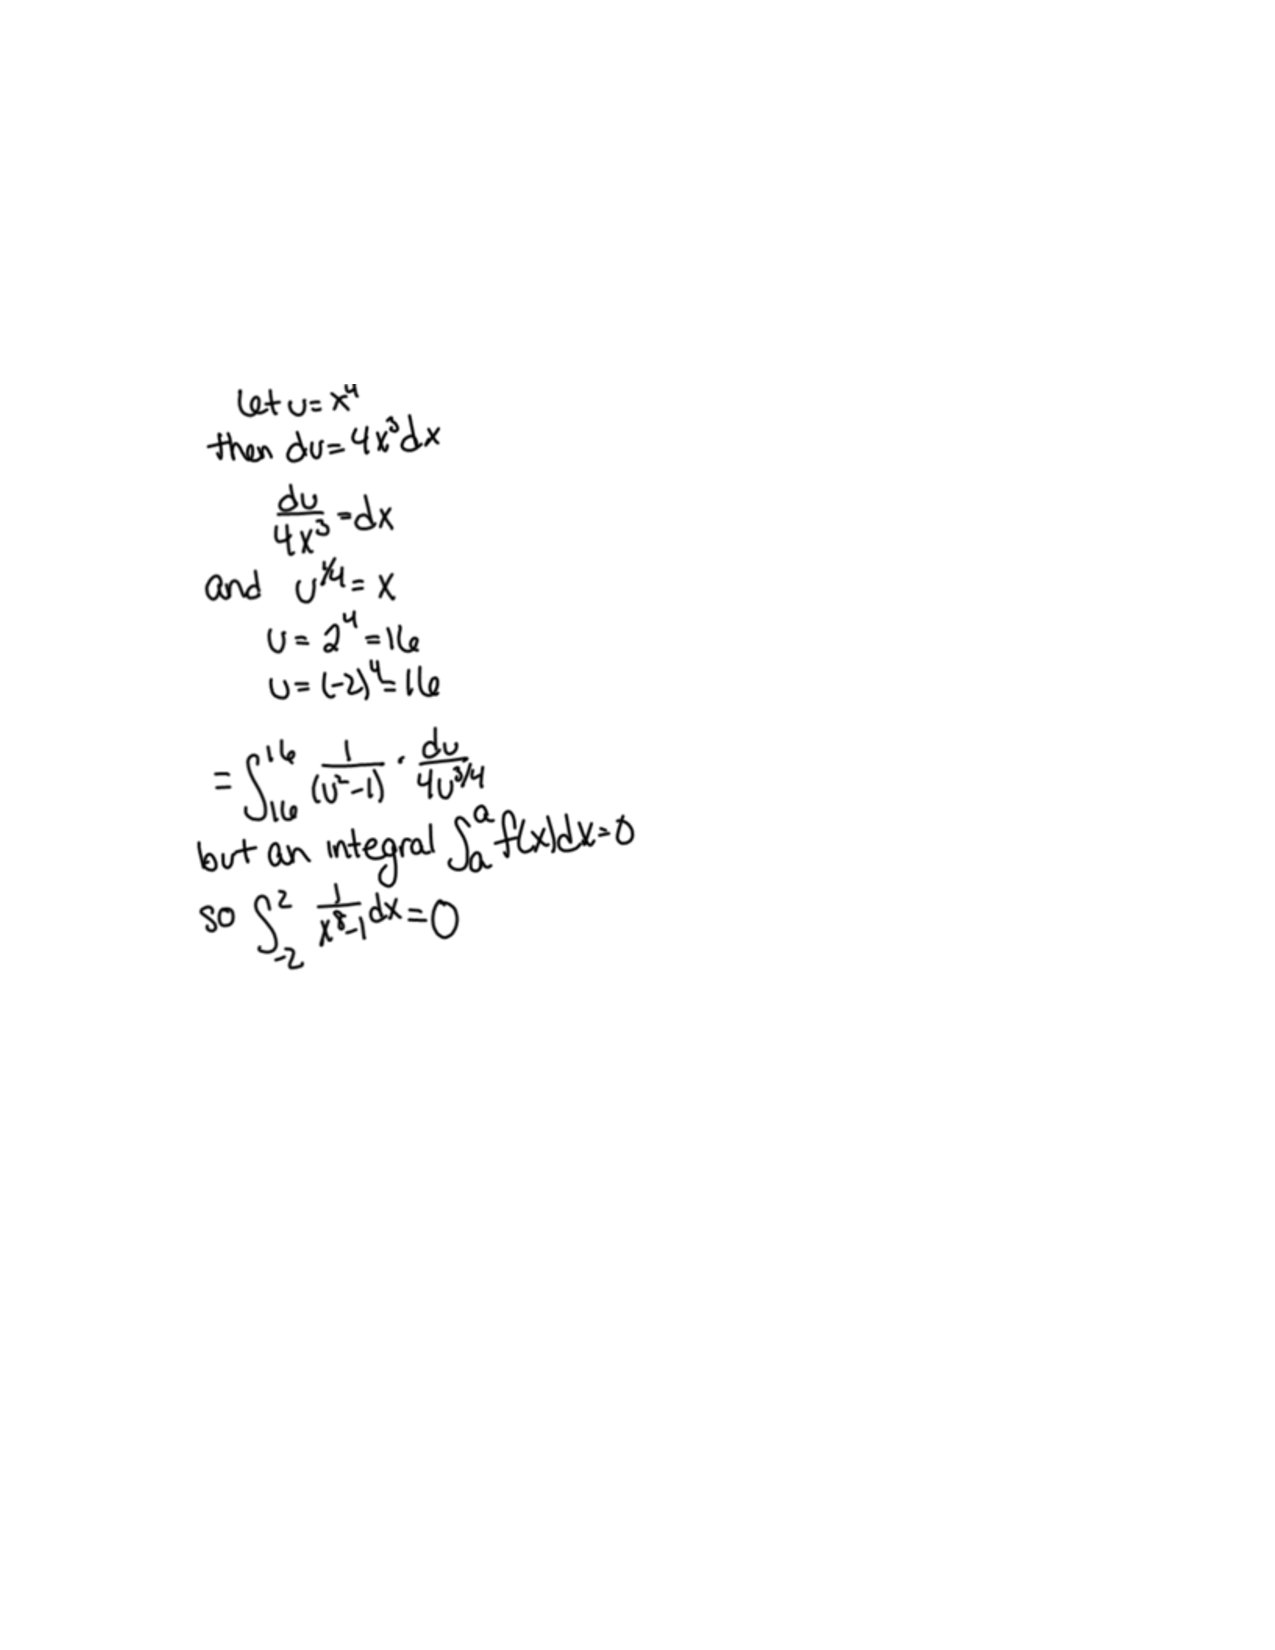
\includegraphics[trim= 170 420 250 180]{Figure1.pdf}
%\end{image}

%add a ``.'' below when used in a specific directory.
\newcommand{\RR}{\mathbb R}
\renewcommand{\d}{\,d}
\newcommand{\dd}[2][]{\frac{d #1}{d #2}}
\renewcommand{\l}{\ell}
\newcommand{\ddx}{\frac{d}{dx}}
\newcommand{\dfn}{\textbf}
\newcommand{\eval}[1]{\bigg[ #1 \bigg]}

\usepackage{multicol}

\renewenvironment{freeResponse}{
\ifhandout\setbox0\vbox\bgroup\else
\begin{trivlist}\item[\hskip \labelsep\bfseries Solution:\hspace{2ex}]
\fi}
{\ifhandout\egroup\else
\end{trivlist}
\fi} %% we can turn off input when making a master document

\title{Section 7.4: Trig Substitution}  

\begin{document}
\begin{abstract}		\end{abstract}
\maketitle



\begin{comment}
\section{Warm up:}

	\begin{freeResponse}
	
	\end{freeResponse}
	
\begin{instructorNotes}

\end{instructorNotes}
\end{comment}


\section{Group work:}

%Problem 1
\begin{problem}
For the integral:
$$\displaystyle \int \frac{27 x^2}{(4+9x^2)^{3/2}} \, \mathrm{d}x$$
find an appropriate constant $C$ and an appropriate trigonometric substitution of one of the forms $x=C \sin \theta$, $x=C \sec \theta$, or $x=C \tan \theta$ to simplify the integral.  Then, perform any  trigonometric manipulations necessary and evaluate the integral.


\end{problem}

%problem 2
\begin{problem}
Evaluate the following integrals:
	\begin{enumerate}
	\item $\displaystyle \int \limits_{ -\frac{5}{3}}^{-\frac{5}{6}} \frac{\sqrt{36x^2-25}}{x^3} \d x$
	\item $\displaystyle \int \frac{\d x}{\left( x^2 - 6x + 11 \right)^2}$
	
	\end{enumerate}

\end{problem}


%problem 3
\begin{problem}
Evaluate the following integrals:
	\begin{enumerate}

		
	\item $\displaystyle \int \frac{x^2}{\sqrt{4x-x^2}} \d x$
	\item $\displaystyle \int \frac{e^x}{\sqrt{e^{2x}+9}} \d x$
	\item $\displaystyle \int \frac{\d x}{x^{\frac{1}{2}} - 9x^{\frac{3}{2}}}$
	
	

	\end{enumerate}

\end{problem}



\end{document} 


















